\chapter{Mitigations against Cache side channels}

Software based mitigations against cache side channels involve changing the
implementation of each encryption algorithm to avoid leaking data. But that is only
possible for a specific set of known attacks, and it is unavoidable for any software
to not leave some kind of fingerprint in the shared resources.

A proper solution involves changing hardware design of caches so that one process
doesn't affect other processes via its cache accesses in a predictable way.

\section{Partition-locked cache}

Cache partitioning is a naive way of isolating processes from interfering with
each other's cache accesses.
A partitioned cache will let only one process access a single partition at a
time \Citeref{part_cache}.
If we partition the cache statically, it is equivalent to having a private
cache for every thread on the core.
This either leads to huge power and area usage or high drop in performance.

Wang et al have proposed a dynamically partitioned cache in \Citeref{
pl_rp_cache}. As seen in \Figref{fig:plcache},
they add extra bits to every cache line to determine whether line is "Locked"
and "ID" of thread which locked it.
A modified cache replacement policy takes into account these bits when
replacing any line.
This ensures that locked lines can only be replaced by the process that locked
them. Hence, other processes will not be able to interfere with locked lines.

\begin{figure}
    \centering
    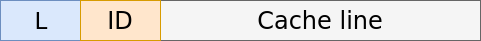
\includegraphics[width=0.7\textwidth]{pl-cache}
    \caption{A single cache line of PLCache}
    \label{fig:plcache}
\end{figure}

For implementing the PLCache, the hardware level changes include extra bits
for every cache line and a change of the replacement policy.
However, PLCache requires addition of special locked-load/store instructions to the ISA.
This also means OS has to look over which process gets to use them as a fairness measure.
If unchecked, attackers can intentionally lock lines which will hinder
performance of other programs.
Overuse or abuse of the locking feature can lead to severe performance
degradation, if not checked by the OS.

PLCache is better than static partitioning in that it allows locked partitions
of the cache to be assigned dynamically.
But it has certain drawbacks in terms of implementation.

\section{Random permutation cache}

Random-permutation cache is another cache design proposed by Wang et al in
\Citeref{pl_rp_cache}.
They have added a redirection step in the address decoder of caches which uses
a random permutation table as seen in \Figref{fig:rpcache}.
The permutation table essentially randomises the cache line in which an
address will be stored.
The size of permutation table is larger than cache size (in terms of number of
lines) such that there is lesser aliasing in the permutation table. Moreover,
the replacement policy is modified to update the permutation table for every
replacement, hence an attacker will not be able to decode the mapping.

\begin{figure}
    \centering
    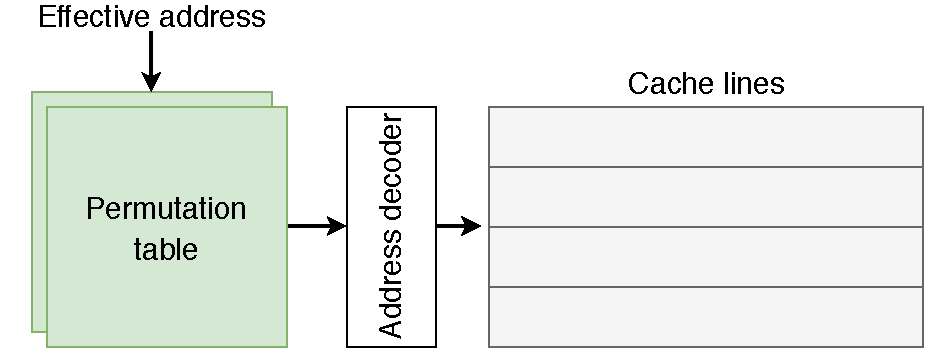
\includegraphics[width=0.7\textwidth]{rp-cache}
    \caption{Address decoding in RPCache}
    \label{fig:rpcache}
\end{figure}

RPcache is also able to mark sensitive data using "Lock" bits which are
derived by page protected bit.
This is possible without any modification to ISA hence it is better than PLCache.
The only drawback of RPCache is the added step in address decoding, which will
increase cache latency by one or two cycles.
This may not affect L2 or L3 caches much but it will drastically change
performance of L1.
To overcome this Wang et al propose optimisations to the gate-level hardware
of the decoder.
The also propose an improved cache architecture called Newcache
\Citeref{newcache} which overcomes these issues while not losing in power and
performance.

\section{Intentional Cache pollution}

Cache pollution happens when unnecessary data resides in cache and evicts
important data which is being used by processes.
It happens generally due to poor design and designers will
try to avoid it as much as possible, by using smarter replacement policies.

From a security perspective, we can use cache pollution to our advantage by
introducing enough noise in a cache side channel such that is hides leaked
information. There are multiple ways of intentionally polluting the cache. Two
such ways are presented below.

\subsection{Disruptive Prefetching} \label{sec:disruptive-section}

\begin{figure}[ht]
    \centering
    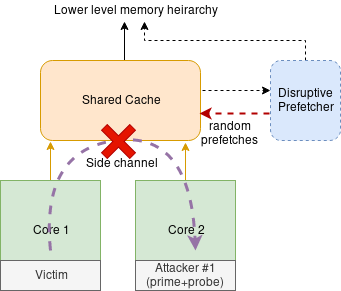
\includegraphics[width=0.5\textwidth]{disruptive_prefetch}
    \caption{Disruptive prefetcher preventing side channel leakage}
    \label{fig:disruptive_prefetch}
\end{figure}

Pre-fetchers are hardware blocks which were originally designed to hide memory
access latency by guessing the need of certain memory address based on
previous memory access patterns. Memory locations guessed by the pre-fetcher
are loaded into cache so that when the code execution requires that memory, it
gives a cache hit instead of miss. Pre-fetchers like Stride pre-fetcher and
GHB pre-fetcher are based on finding patterns in the previous memory accesses
and guessing that the next locations in that pattern will be accessed. Fuchs
et al in \Citeref{disruptive} introduce additional steps to the prefetchers
to increase the randomness in the memor access pattern. They randomise the
pattern sequence and degree of prefetching to intentionally pollute the cache with
unnecessary data. This will degrade the performance of non-malicious programs
by a bit, but will terribly disrupt any side channel established by an
attacker. For example, in Prime+Probe attack, the attacker will not know
whether the victim or the pre-fetcher evicted its block from the cache, hence
it will wrongly trace the memory access of the victim. In the same way,
Flush+Reload would get false cache hits which were not caused by the victim.

In \Figref{fig:disruptive_prefetch}, there is a side channel established
between Victim and Attacker process. The shared cache has a disruptive
prefetcher which is continuously introducing random prefetches on every access
(prefetcher hit or miss). This is causing the Prime+Probe attack to detect
other cache locations which  were not accessed by the victim but because of
these random prefetches.

\subsection{Context sensitive decoding}

A lot of modern processors use decoders to convert from ISA to an internal
instruction representation. Most popularly Intel converts from x86 ISA to
microcode using a microcode cache mapping table. Taram et al explore in
\Citeref{csd} if a custom decoder can be used to improve the security of
certain programs. They use the decoder to introduce decoy instructions in the
pipeline. These decoy instructions will change the timing characteristics of
the executing program, they will pollute the cache by running decoy loads and
will disrupt attackers attempting side channel or timing attacks. Their
implementation, as seen in \Figref{fig:csd} includes adding custom decoder
hardware, and a few changes to the microcode mapping table (of which there
exists an established update procedure), and a few model specific registers to
control the context of the program. They show their method to be effective in
stopping I-Cache and D-Cache side channel attacks against RSA and AES.

\begin{figure}[hb]
    \centering
    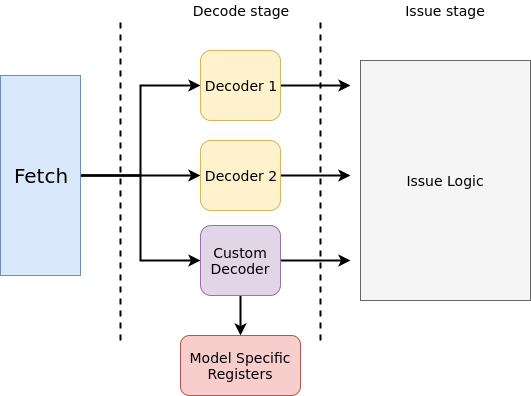
\includegraphics[width=0.7\textwidth]{csd}
    \caption{Custom decoder for context sensitive decoding}
    \label{fig:csd}
\end{figure}

